\thispagestyle{plain}

\section{Results}

In addition to  classification accuracy, relative increase of this metric with respect to the previous one is displayed on Table~\ref{tableacc}. Random choice, as expected, performed worse with 50\% accuracy, followed by a significant increase with TF-IDF vectorization. CBOW embeddings slightly improved accuracy up to 81\%. DistilBERT embeddings achieve the highest accuracy, 86\%, a 6.2\% increase from CBOW and a 72\% increase relative to the dummy classifier. These results are also reflected in Figure~\ref{cm} where the confusion matrices for all methods are displayed.

\begin{table}[h]
	\centering
	\resizebox{7cm}{!}{%
		\begin{tabular}{lcc}
			\hline
			\multicolumn{1}{c}{Method} & Accuracy & Relative increase \\ \hline
			Random choice              & 0.5      & 0\%               \\ 
			TF-IDF                     & 0.79     & 58\%              \\ 
			CBOW                       & 0.81     & 2.5\%             \\ 
			distilBERT                 & 0.86     & 6.2\%             \\ \hline
		\end{tabular}%
	}
\caption{Accuracy for different vectorization/embeddings.}
\label{tableacc}
\end{table}



\begin{figure}[h]
	\begin{tabular}{cc}
		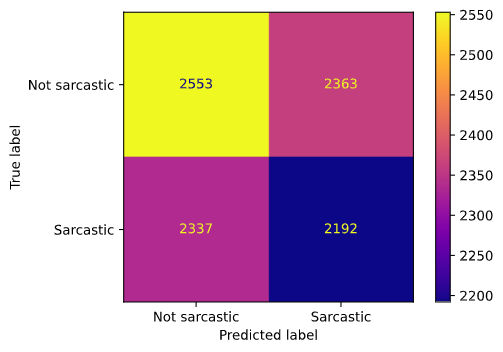
\includegraphics[width=70mm]{../img/dummy-cm.png}\label{cmrandom} &   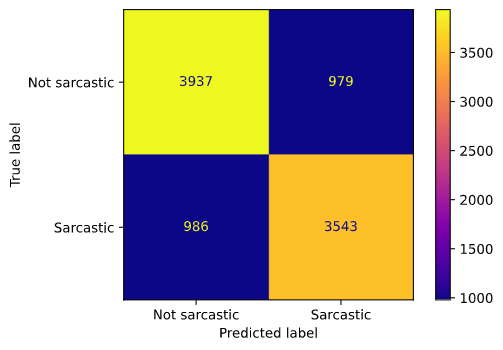
\includegraphics[width=70mm]{../img/tfidf-cm.png}\label{cmtfidf} \\
		(a) Random choice & (b) TF-IDF \\[6pt]
		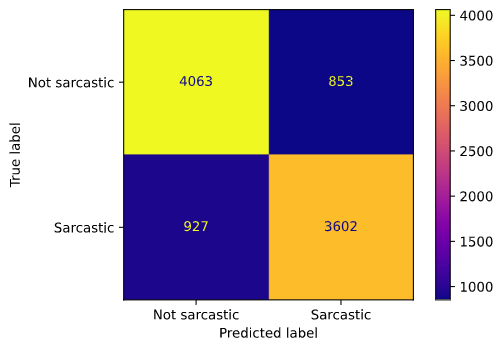
\includegraphics[width=70mm]{../img/w2v-cm.png}\label{cmcbow} &   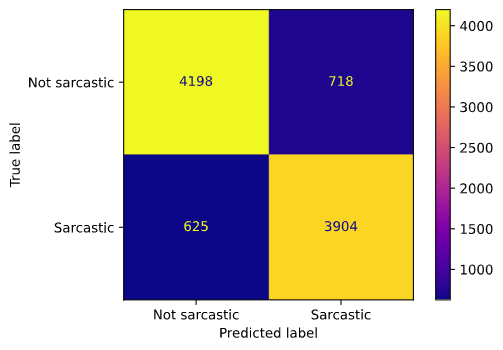
\includegraphics[width=70mm]{../img/bert-cm.png}\label{cmdistilbert} \\
		(c) CBOW & (d) distilBERT \\[6pt]
	\end{tabular}
	
	\caption{Confusion matrices}
	\label{cm}
\end{figure}